%%
%%

\section*{Getting Started with Bacula}
\label{_ChapterStart37}
\index[general]{Getting Started with Bacula }
\addcontentsline{toc}{section}{Getting Started with Bacula}

If you are like me, you want to get Bacula running immediately to get a feel
for it, then later you want to go back and read about all the details. This
chapter attempts to accomplish just that: get you going quickly without all
the details. If you want to skip the section on Pools, Volumes and Labels, you
can always come back to it, but please read to the end of this chapter, and in
particular follow the instructions for testing your tape drive. 

We assume that you have managed to build and install Bacula, if not, you might
want to first look at the 
\ilink{System Requirements}{SysReqs} then at the 
\ilink{Compiling and Installing Bacula}{_ChapterStart17} chapter of
this manual. 
\label{PoolsVolsLabels}

\subsection*{Understanding Pools, Volumes and Labels}
\index[general]{Labels!Understanding Pools Volumes and }
\index[general]{Understanding Pools, Volumes and Labels }
\addcontentsline{toc}{subsection}{Understanding Pools, Volumes and Labels}

If you have been using a program such as {\bf tar} to backup your system,
Pools, Volumes, and labeling may be a bit confusing at first. A Volume is a
single physical tape (or possibly a single file) on which Bacula will write
your backup data. Pools group together Volumes so that a backup is not
restricted to the length of a single Volume (tape). Consequently, rather than
explicitly naming Volumes in your Job, you specify a Pool, and Bacula will
select the next appendable Volume from the Pool and request you to mount it. 

Although the basic Pool options are specified in the Director's Pool resource,
the {\bf real} Pool is maintained in the Bacula Catalog. It contains
information taken from the Pool resource (bacula-dir.conf) as well as
information on all the Volumes that have been added to the Pool. Adding
Volumes to a Pool is usually done manually with the Console program using the
{\bf label} command. 

For each Volume, Bacula maintains a fair amount of catalog information such as
the first write date/time, the last write date/time, the number of files on
the Volume, the number of bytes on the Volume, the number of Mounts, etc. 

Before Bacula will read or write a Volume, the physical Volume must have a
Bacula software label so that Bacula can be sure the correct Volume is
mounted. This is usually done using the {\bf label} command in the Console
program. 

The steps for creating a Pool, adding Volumes to it, and writing software
labels to the Volumes, may seem tedious at first, but in fact, they are quite
simple to do, and they allow you to use multiple Volumes (rather than being
limited to the size of a single tape). Pools also give you significant
flexibility in your backup process. For example, you can have a ``Daily'' Pool
of Volumes for Incremental backups and a ``Weekly'' Pool of Volumes for Full
backups. By specifying the appropriate Pool in the daily and weekly backup
Jobs, you thereby insure that no daily Job ever writes to a Volume in the
Weekly Pool and vice versa, and Bacula will tell you what tape is needed and
when. 

For more on Pools, see the 
\ilink{Pool Resource}{PoolResource} section of the Director
Configuration chapter, or simply read on, and we will come back to this
subject later. 

\subsection*{Setting Up Bacula Configuration Files}
\label{config}
\index[general]{Setting Up Bacula Configuration Files }
\index[general]{Files!Setting Up Bacula Configuration }
\addcontentsline{toc}{subsection}{Setting Up Bacula Configuration Files}

After running the appropriate {\bf ./configure} command and doing a {\bf
make}, and a {\bf make install}, if this is the first time you are running
Bacula, you must create valid configuration files for the Director, the File
daemon, the Storage daemon, and the Console programs. If you have followed our
recommendations, default configuration files as well as the daemon binaries
will be located in your installation directory. In any case, the binaries are
found in the directory you specified on the {\bf \verb{--{sbindir} option to the {\bf
./configure} command, and the configuration files are found in the directory
you specified on the {\bf \verb{--{sysconfdir} option. 

When initially setting up Bacula you will need to invest a bit of time in
modifying the default configuration files to suit your environment. This may
entail starting and stopping Bacula a number of times until you get everything
right. Please do not despair. Once you have created your configuration files,
you will rarely need to change them nor will you stop and start Bacula very
often. Most of the work will simply be in changing the tape when it is full. 

\subsubsection*{
\ilink{Configuring the Console Program}{_ChapterStart36}}
\index[general]{Configuring the Console Program }
\index[general]{Program!Configuring the Console }
\addcontentsline{toc}{subsubsection}{Configuring the Console Program}

The Console program is used by the administrator to interact with the Director
and to manually start/stop Jobs or to obtain Job status information. 

The Console configuration file is found in the directory specified on the {\bf
\verb{--{sysconfdir} option that you specified on the {\bf ./configure} command and
by default is named {\bf console.conf}.

If you choose to build the GNOME console with the {\bf \verb{--{enable-gnome} option,
you also find a default configuration file for it, named {\bf
gnome-console.conf}.

The same applies to the wxWidgets console, which is build with the {\bf
\verb{--{enable-wx-console} option, and the name of the default configuration file
is, in this case, {\bf wx-console.conf}.

Normally, for first time users, no change is needed to these files. Reasonable
defaults are set. 

\subsubsection*{
\ilink{Configuring the Monitor Program}{_ChapterStart35}}
\index[general]{Program!Configuring the Monitor }
\index[general]{Configuring the Monitor Program }
\addcontentsline{toc}{subsubsection}{Configuring the Monitor Program}

The Monitor program is typically an icon in the system tray. However, once the
icon is expanded into a full window, the administrator or user can obtain
status information about the Director or the backup status on the local
workstation or any other Bacula daemon that is configured. 

\addcontentsline{lof}{figure}{Bacula Tray Monitor}
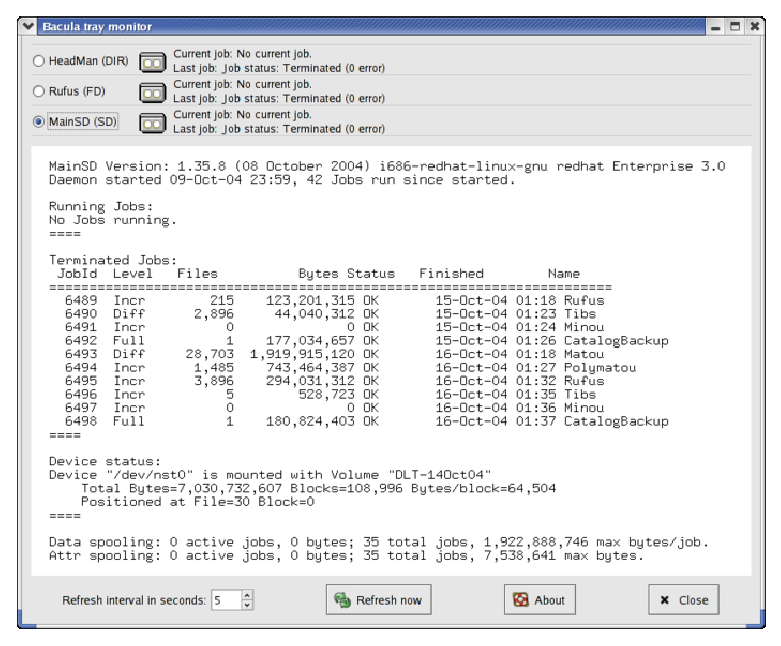
\includegraphics{./Bacula-tray-monitor.eps} 

The image shows a tray-monitor configured for three daemons. By clicking on
the radio buttons in the upper left corner of the image, you can see the
status for each of the daemons. The image shows the status for the Storage
daemon (MainSD) that is currently selected. 

The Monitor configuration file is found in the directory specified on the {\bf
\verb{--{sysconfdir} option that you specified on the {\bf ./configure} command and
by default is named {\bf tray-monitor.conf}. Normally, for first time users,
you just need to change the permission of this file to allow non-root users to
run the Monitor, as this application must run as the same user as the
graphical environment (don't forget allow non-root users to execute {\bf
bacula-tray-monitor}). This is not a security problem as long as you use the
default settings. 

\subsubsection*{
\ilink{Configuring the File daemon}{_ChapterStart25}}
\index[general]{Daemon!Configuring the File }
\index[general]{Configuring the File daemon }
\addcontentsline{toc}{subsubsection}{Configuring the File daemon}

The File daemon is a program that runs on each (Client) machine. At the
request of the Director, finds the files to be backed up and sends them (their
data) to the Storage daemon. 

The File daemon configuration file is found in the directory specified on the
{\bf \verb{--{sysconfdir} option that you specified on the {\bf ./configure} command.
By default, the File daemon's configuration file is named {\bf
bacula-fd.conf}. Normally, for first time users, no change is needed to this
file. Reasonable defaults are set. However, if you are going to back up more
than one machine, you will need to install the File daemon with a unique
configuration file on each machine to be backed up. The information about each
File daemon must appear in the Director's configuration file. 

\subsubsection*{
\ilink{Configuring the Director}{_ChapterStart40}}
\index[general]{Director!Configuring the }
\index[general]{Configuring the Director }
\addcontentsline{toc}{subsubsection}{Configuring the Director}

The Director is the central control program for all the other daemons. It
schedules and monitors all jobs to be backed up. 

The Director configuration file is found in the directory specified on the
{\bf \verb{--{sysconfdir} option that you specified on the {\bf ./configure} command.
Normally the Director's configuration file is named {\bf bacula-dir.conf}. 

In general, the only change you must make is modify the FileSet resource so
that the {\bf Include} configuration directive contains at least one line with
a valid name of a directory (or file) to be saved. 

If you do not have a DLT tape drive, you will probably want to edit the
Storage resource to contain names that are more representative of your actual
storage device. You can always use the existing names as you are free to
arbitrarily assign them, but they must agree with the corresponding names in
the Storage daemon's configuration file. 

You may also want to change the email address for notification from the
default {\bf root} to your email address. 

Finally, if you have multiple systems to be backed up, you will need a
separate File daemon or Client specification for each system, specifying its
name, address, and password. We have found that giving your daemons the same
name as your system but post fixed with {\bf -fd} helps a lot in debugging.
That is, if your system name is {\bf foobaz}, you would give the File daemon
the name {\bf foobaz-fd}. For the Director, you might use {\bf foobaz-dir},
and for the storage daemon, you might use {\bf foobaz-sd}. 

\subsubsection*{
\ilink{Configuring the Storage daemon}{_ChapterStart31}}
\index[general]{Daemon!Configuring the Storage }
\index[general]{Configuring the Storage daemon }
\addcontentsline{toc}{subsubsection}{Configuring the Storage daemon}

The Storage daemon is responsible, at the Director's request, for accepting
data from a File daemon and placing it on Storage media, or in the case of a
restore request, to find the data and send it to the File daemon. 

The Storage daemon's configuration file is found in the directory specified on
the {\bf \verb{--{sysconfdir} option that you specified on the {\bf ./configure}
command. By default, the Storage daemon's file is named {\bf bacula-sd.conf}.
Edit this file to contain the correct Archive device names for any tape
devices that you have. If the configuration process properly detected your
system, they will already be correctly set. These Storage resource name and
Media Type must be the same as the corresponding ones in the Director's
configuration file {\bf bacula-dir.conf}. If you want to backup to a file
instead of a tape, the Archive device must point to a directory in which the
Volumes will be created as files when you label the Volume. 
\label{ConfigTesting}

\subsection*{Testing your Configuration Files}
\index[general]{Testing your Configuration Files }
\index[general]{Files!Testing your Configuration }
\addcontentsline{toc}{subsection}{Testing your Configuration Files}

You can test if your configuration file is syntactically correct by running
the appropriate daemon with the {\bf -t} option. The daemon will process the
configuration file and print any error messages then terminate. For example,
assuming you have installed your binaries and configuration files in the same
directory. 

\footnotesize
\begin{verbatim}
cd <installation-directory>
./bacula-dir -t -c bacula-dir.conf
./bacula-fd -t -c bacula-fd.conf
./bacula-sd -t -c bacula-sd.conf
./bconsole -t -c bconsole.conf
./gnome-console -t -c gnome-console.conf
./wx-console -t -c wx-console.conf
su <normal user> -c "./bacula-tray-monitor -t -c tray-monitor.conf"
\end{verbatim}
\normalsize

will test the configuration files of each of the main programs. If the
configuration file is OK, the program will terminate without printing
anything. Please note that, depending on the configure options you choose,
some, or even all, of the three last commands will not be available on your
system. If you have installed the binaries in traditional Unix locations
rather than a single file, you will need to modify the above commands
appropriately (no ./ in front of the command name, and a path in front of the
conf file name). 
\label{TapeTesting}

\subsection*{Testing Bacula Compatibility with Your Tape Drive}
\index[general]{Drive!Testing Bacula Compatibility with Your Tape }
\index[general]{Testing Bacula Compatibility with Your Tape Drive }
\addcontentsline{toc}{subsection}{Testing Bacula Compatibility with Your Tape
Drive}

Before spending a lot of time on Bacula only to find that it doesn't work with
your tape drive, please read the 
\ilink{btape -- Testing Your Tape Drive}{_ChapterStart27}
chapter of this manual. If you have a modern standard SCSI tape drive on a
Linux or Solaris, most likely it will work, but better test than be sorry. For
FreeBSD (and probably other xBSD flavors), reading the above mentioned tape
testing chapter is a must. Also, for FreeBSD, please see 
\elink{The FreeBSD Diary}{http://www.freebsddiary.org/bacula.php} for a
detailed description on how to make Bacula work on your system. In addition,
users of FreeBSD prior to 4.9-STABLE dated Mon Dec 29 15:18:01 2003 UTC who
plan to use tape devices, please see the file {\bf
platforms/freebsd/pthreads-fix.txt} in the main Bacula directory concerning
important information concerning compatibility of Bacula and your system. 
\label{notls}

\subsection*{Get Rid of the /lib/tls Directory}
\index[general]{Directory!Get Rid of the /lib/tls }
\index[general]{Get Rid of the /lib/tls Directory }
\addcontentsline{toc}{subsection}{Get Rid of the /lib/tls Directory}

The new pthreads library {\bf /lib/tls} installed by default on recent Red Hat
systems running kernel 2.4.x is defective. You must remove it or rename it
then reboot your system before running Bacula otherwise after a week or so of
running, Bacula will either block for long periods or deadlock entirely. The
feedback that we have concerning 2.6 kernels is the same. However, on 2.6
systems, you may want to use the loader environment variable override rather
than removing /lib/tls. Please see 
\ilink{ Supported Operating Systems}{SupportedOSes} for more
information on this problem. 
\label{Running1}

\subsection*{Running Bacula}
\index[general]{Bacula!Running }
\index[general]{Running Bacula }
\addcontentsline{toc}{subsection}{Running Bacula}

Probably the most important part of running Bacula is being able to restore
files. If you haven't tried recovering files at least once, when you actually
have to do it, you will be under a lot more pressure, and prone to make
errors, than if you had already tried it once. 

To get a good idea how to use Bacula in a short time, we {\bf strongly}
recommend that you follow the example in the 
\ilink{Running Bacula Chapter}{_ChapterStart1} of this manual where
you will get detailed instructions on how to run Bacula. 

\subsection*{Log Rotation}
\index[general]{Rotation!Log }
\index[general]{Log Rotation }
\addcontentsline{toc}{subsection}{Log Rotation}

If you use the default {\bf bacula-dir.conf} or some variation of it, you will
note that it logs all the Bacula output to a file. To avoid that this file
grows without limit, we recommend that you copy the file {\bf logrotate} from
the {\bf scripts/logrotate} to {\bf /etc/logrotate.d/bacula}. This will cause
the log file to be rotated once a month and kept for a maximum of 5 months.
You may want to edit this file to change the default log rotation preferences.


\subsection*{Disaster Recovery}
\index[general]{Recovery!Disaster }
\index[general]{Disaster Recovery }
\addcontentsline{toc}{subsection}{Disaster Recovery}

If you intend to use Bacula as a disaster recovery tool rather than simply a
program to restore lost or damaged files, you will want to read the 
\ilink{Disaster Recovery Using Bacula Chapter}{_ChapterStart38} of
this manual. 

In any case, you are strongly urged to carefully test restoring some files
that you have saved rather than wait until disaster strikes. This way, you
will be prepared. 
